%dip.tex
\documentclass{article}
%page
\usepackage{geometry}
\geometry{a4paper,centering,scale=0.8}
%\geometry{a4paper,left=3cm,right=3cm}

\usepackage{fancyhdr}
\pagestyle{fancy}
\fancyhf{} %清空所有的页眉页脚
\cfoot{\thepage}
\lhead{
\includegraphics[scale=0.03]{nanhang.png} 南京航空航天大学}
\rhead{模式识别实验报告}
\usepackage[BoldFont,SlantFont,CJKchecksingle]{xeCJK}

%chinese
\usepackage{ctex}


%the set of coding
\usepackage{listings}
\usepackage{color}
\definecolor{mygreen}{rgb}{0.48,0.77,0.8}
\definecolor{mygray}{rgb}{0.5,0.5,0.5}
\definecolor{mymauve}{rgb}{0.8,0,0}
\lstset{ %
  backgroundcolor=\color{white},   % choose the background color; you must add \usepackage{color} or \usepackage{xcolor}; should come as last argument
  basicstyle=\footnotesize,        % the size of the fonts that are used for the code
  breakatwhitespace=false,         % sets if automatic breaks should only happen at whitespace
  breaklines=true,                 % sets automatic line breaking
  captionpos=k,                    % sets the caption-position to bottom
  commentstyle=\color{mygreen},    % comment style
  deletekeywords={...},            % if you want to delete keywords from the given language
  escapeinside={\%*}{*)},          % if you want to add LaTeX within your code
  extendedchars=true,              % lets you use non-ASCII characters; for 8-bits encodings only, does not work with UTF-8
  frame=single,	                   % adds a frame around the code
  keepspaces=true,                 % keeps spaces in text, useful for keeping indentation of code (possibly needs columns=flexible)
  keywordstyle=\color{blue},       % keyword style
  language=Octave,                 % the language of the code
  morekeywords={*,...},           % if you want to add more keywords to the set
  numbers=left,                    % where to put the line-numbers; possible values are (none, left, right)
  numbersep=5pt,                   % how far the line-numbers are from the code
  numberstyle=\tiny\color{mygray}, % the style that is used for the line-numbers
  rulecolor=\color{black},         % if not set, the frame-color may be changed on line-breaks within not-black text (e.g. comments (green here))
  showspaces=false,                % show spaces everywhere adding particular underscores; it overrides 'showstringspaces'
  showstringspaces=false,          % underline spaces within strings only
  showtabs=false,                  % show tabs within strings adding particular underscores
  stepnumber=2,                    % the step between two line-numbers. If it's 1, each line will be numbered
  stringstyle=\color{mymauve},     % string literal style
  tabsize=2,	                   % sets default tabsize to 2 spaces
  title=\lstname                   % show the filename of files included with \lstinputlisting; also try caption instead of title
}

%float
\usepackage{float}
%draw picture
\usepackage{graphics}
%abreast
\usepackage{subfigure}

\renewcommand{\thefigure}{\thesection.\arabic{figure}} % set caption label style to 1.A

%\setCJKmainfont[BoldFont=SimHei]{SimSun}%设置\rmfamily

\title{\textbf{\zihao{2}模式识别实验报告\\ }}   
\author{161440110 张涛,1614402 姚韫玉}
\date{\today}

%links
\usepackage[colorlinks,linkcolor=red]{hyperref}
\usepackage{tabularx}

%---------------------正文--------
\begin{document}

	%-----------reference
\bibliographystyle{plain}
	%-----------题目
\maketitle
\begin{abstract}
模式识别是在某些一定量度或观测基础上把待识模式划分到各自的模式类中去。计算机模式识别就是指利用计算机等装置对物体,图像等信息进行自动的识别。
实验使用mnist数据集和iris数据集,分类算法使用传统的卷积神经网络模型模型cnn和最近hinton提出的capsule算法。比较两者在mnist数据集上的表现。聚类算法使用k-means和混合高斯分布GMM在iris数据集上做聚类,比较两个算法在此数据集上的表现
\end{abstract}
	%-----------正文
\section{数据集介绍}
实验采用的数据集是机器学习领域最基础的两个数据集,也是很多实验中常用的数据集,本次使用也使用这两个数据集作为基准,比较分类和聚类算法的性能。
\subsection{mnist\cite{mnist}}
MNIST数据集可在\url{http://yann.lecun.com/exdb/mnist/}获取,它包含了四个部分:
\begin{itemize}
	\item Training set images: train-images-idx3-ubyte.gz (9.9 MB, 解压后 47 MB, 包含 60,000 个样本)
    \item Training set labels: train-labels-idx1-ubyte.gz (29 KB, 解压后 60 KB, 包含 60,000 个标签)
    \item Test set images: t10k-images-idx3-ubyte.gz (1.6 MB, 解压后 7.8 MB, 包含 10,000 个样本)
    \item Test set labels: t10k-labels-idx1-ubyte.gz (5KB, 解压后 10 KB, 包含 10,000 个标签)
\end{itemize}

数据是28*28的图片,图片中是手写体的数字。每张图片都有对应的类标,表示图片上的数字是几,如图所示
\begin{figure}[htbp]
\centering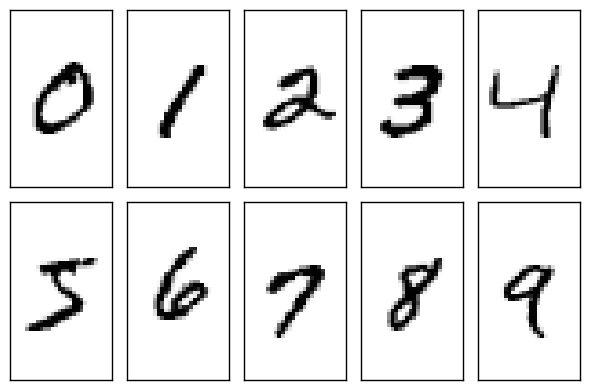
\includegraphics[scale=0.6]{mnist}
\caption{mnist图片示意}\label{fig:1}
\end{figure}
任务就是训练模型,识别图片中的数据。

\subsection{iris}
Iris也称鸢尾花卉数据集,是一类多重变量分析的数据集。通过花萼长度,花萼宽度,花瓣长度,花瓣宽度4个属性预测鸢尾花卉属于(Setosa,Versicolour,Virginica)三个种类中的哪一类。

\begin{table}

\begin{tabularx}{\textwidth}{|X|X|X|X|}
\hline
\textbf{数据集特征:} & 多变量 & \textbf{记录数:} & 150 \\
\hline
\textbf{属性特征:} & 实数 & \textbf{属性数目:} & 4 \\
\hline
\textbf{相关应用:} & 分类 & \textbf{缺失值?} & 无 \\
\hline
\end{tabularx}
\caption{iris数据属性介绍}
\end{table}


\section{算法介绍}
	\subsection{分类算法}
	分类算法是处理有标签数据的问题,在测试集上训练模型,然后在测试集上结合真实类标评估分类算法的性能。下面的实验中是使用mnist数据集。
	\subsubsection{convolution neural network}
	\textbf{卷积神经网络(Convolutional Neural Network,CNN)}[1]是一种前馈神经网络,它的人工神经元可以响应一部分覆盖范围内的周围单元,对于大型图像处理有出色表现.它包括卷积层(convolutional layer)和池化层(pooling layer).卷积神经网络是近年发展起来,并引起广泛重视的一种高效识别方法.
	\begin{figure}[htbp]
	\centering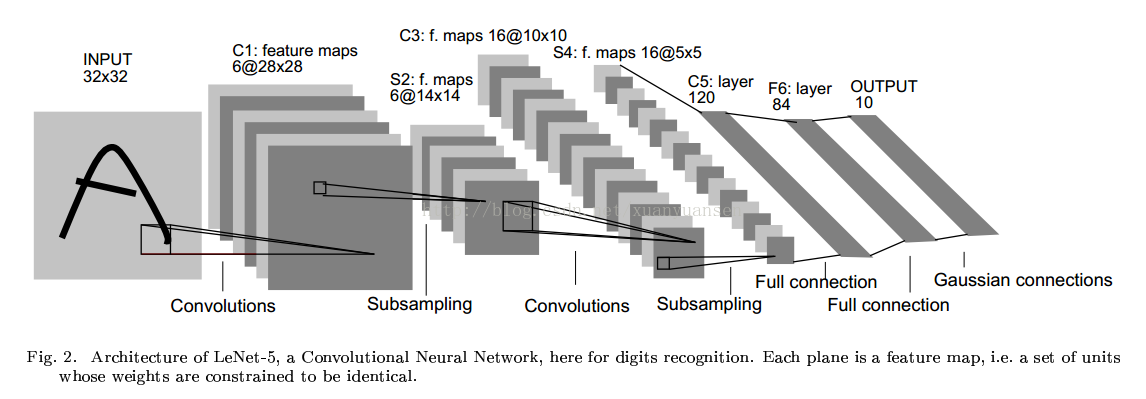
\includegraphics[scale=0.6]{cnn}
	\caption{LeNet5}\label{fig:2}
	\end{figure}
	\subsubsection{capsule}
	Capsule 是一组神经元,其输入输出向量表示特定实体类型的实例化参数(即特定物体、概念实体等出现的概率与某些属性)。我们使用输入输出向量的长度表征实体存在的概率,向量的方向表示实例化参数(即实体的某些图形属性)。同一层级的 capsule 通过变换矩阵对更高级别的 capsule 的实例化参数进行预测。当多个预测一致时(本论文使用动态路由使预测一致),更高级别的 capsule 将变得活跃。
	
	Capsule 中的神经元的激活情况表示了图像中存在的特定实体的各种性质。这些性质可以包含很多种不同的参数,例如姿势(位置,大小,方向)、变形、速度、反射率,色彩、纹理等等。而输入输出向量的长度表示了某个实体出现的概率,所以它的值必须在 0 到 1 之间
	
	\begin{figure}[htbp]
	\centering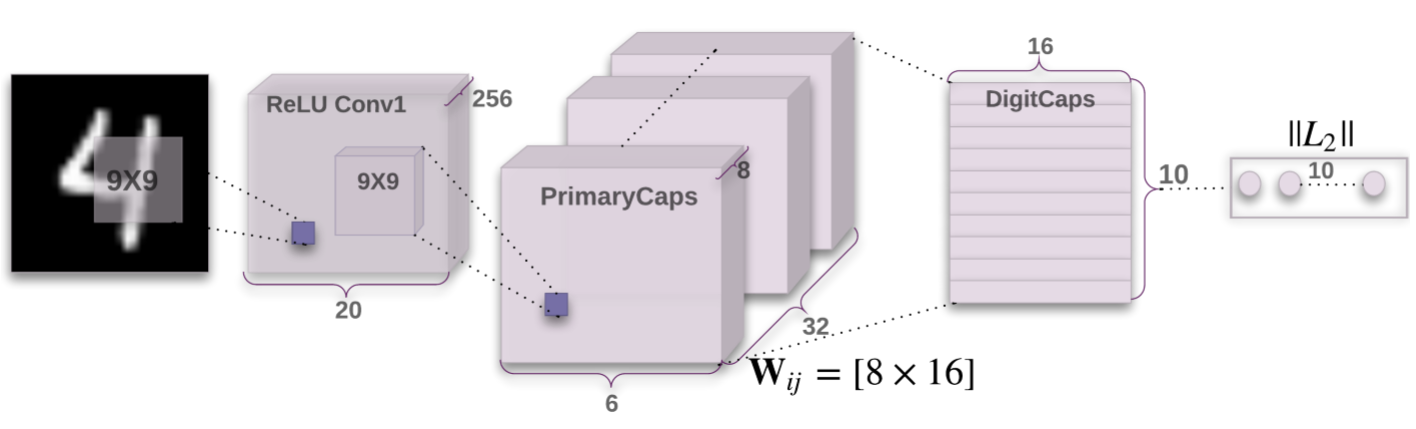
\includegraphics[scale=0.3]{capsule}
	\caption{capsule结构}\label{fig:3}
	\end{figure}
	\subsection{聚类算法}
	聚类算法是一类无标签数据处理的方式,将所有的无标签数据根据不同的属性分成不同的类,本实验使用iris数据集,使用聚类算法进行分类,然后通过真实标签,评估不同的聚类算法的表现性能
	\subsubsection{k-means}
	K-means算法是很典型的基于距离的聚类算法,采用距离作为相似性的评价指标,即认为两个对象的距离越近,其相似度就越大。该算法认为簇是由距离靠近的对象组成的,因此把得到紧凑且独立的簇作为最终目标。
	
	k个初始类聚类中心点的选取对聚类结果具有较大的影响,因为在该算法第一步中是随机的选取任意k个对象作为初始聚类的中心,初始地代表一个簇。该算法在每次迭代中对数据集中剩余的每个对象,根据其与各个簇中心的距离将每个对象重新赋给最近的簇。当考察完所有数据对象后,一次迭代运算完成,新的聚类中心被计算出来。如果在一次迭代前后,J的值没有发生变化,说明算法已经收敛。
	\subsubsection{GMM}
	高斯模型就是用高斯概率密度函数(正态分布曲线)精确地量化事物,将一个事物分解为若干的基于高斯概率密度函数(正态分布曲线)形成的模型。

\section{实验结果}
\subsection{分类算法实验}
\subsection{聚类算法实验}
\bibliography{reference}

\end{document}